\documentclass[11pt,a4paper]{article}
\usepackage[margin=2.0cm]{geometry}
\usepackage{graphicx,booktabs,amsmath}
\usepackage[colorlinks=true,linkcolor=blue,urlcolor=blue]{hyperref}
\setlength{\parskip}{0.45em}
\setlength{\parindent}{0pt}
\newcommand{\FT}{\mathcal{F}}
\begin{document}

\textbf{\large The forward model, and three sweeps that test it}

\textit{Fluo-BPM, at the optics of \texttt{confocal\_emf3.czi}. 2026-08-05}

\section*{1. The model, in one page}

\textbf{Propagation.} Maxwell's equations for a monochromatic scalar field in a
non-magnetic medium reduce to the Helmholtz equation
\begin{equation}
\nabla^2 U(\vec r) + k(\vec r)^2 U(\vec r) = 0,
\qquad k(\vec r) = \frac{2\pi n(\vec r)}{\lambda},
\end{equation}
which keeps the full three-dimensional index distribution $n(\vec r)$ but drops
polarization. Splitting the index into a background $n_0$ and a deviation
$\delta n = n - n_0$, and keeping only forward propagation, the volume is treated as
$P$ slices of thickness $\Delta z$, each carrying a phase map
$\phi_k(x,y) = 2\pi \delta n_k(x,y) \Delta z / \lambda$. One slice to the next is then
\begin{equation}
U_{k+1} = \FT^{-1}\!\Big[\;\FT\big[\,U_k \, e^{i\phi_k}\,\big] \odot \tilde H_{\Delta z}\;\Big],
\qquad
\tilde H_{\Delta z}(\mu_x,\mu_y) = e^{\,i 2\pi \Delta z \sqrt{n_0^2/\lambda^2 - \mu_x^2 - \mu_y^2}} ,
\label{eq:bpm}
\end{equation}
a phase multiplication for what the light passes through, then a Fresnel propagation
for how it diffracts on the way to the next slice. $\odot$ is point-wise
multiplication. Equation~\eqref{eq:bpm} is the whole propagation engine; everything
else is what is put into it and what is read out of it.

\textbf{Fluorescent sources.} Emitters add a source term, and their incoherence is the
statement that different points are uncorrelated,
\begin{equation}
\mathbb{E}\big[s^*(\vec r\,')\,s(\vec r)\big] = \delta(\vec r\,' - \vec r)\, F(\vec r),
\end{equation}
with $F$ the fluorophore distribution. The measured intensity is then
$I(\vec r\,') = \int |G(\vec r\,',\vec r)|^2 F(\vec r)\, d\vec r$, where $G$ is the
Green function that Eq.~\eqref{eq:bpm} implements. That integral has no closed form,
because it needs $|G|^2$ rather than $G$. It can, however, be sampled: drawing a
random phase $\psi \sim \mathcal{U}[0, 2\pi]$ per emitter and propagating the
\emph{coherent} field $\sqrt{F}\,e^{i\psi}$ gives
\begin{equation}
I = \mathbb{E}_\psi\Big[\;\big|\,G\,\big(\sqrt{F} \odot e^{i\psi}\big)\,\big|^2\;\Big],
\label{eq:mc}
\end{equation}
since a diagonal source covariance is exactly what that draw produces:
$\Gamma_U = G\,\Gamma_S\,G^H$ with $\Gamma_S = \mathrm{diag}(F)$ gives
$\Gamma_{U,ii} = \sum_j |G_{ij}|^2 F_j = I_i$. \emph{Incoherent light is thus
simulated as an average of coherent propagations.} In the slice recursion, with
$w = 1 \ldots W$ indexing the draws,
\begin{equation}
U_{k+1,w} = \FT^{-1}\bigg[\;\FT\Big[\;U_{k,w}\,e^{i\phi_k}
 \;+\; \FT^{-1}\big[\,\FT[\,\sqrt{F_k}\,e^{i\psi_{k,w}}\,] \odot C^{-1}\big]\;\Big]
 \odot \tilde H_{\Delta z}\;\bigg],
\label{eq:src}
\end{equation}
where $C = \sqrt{n_0^2/\lambda^2 - \mu_x^2 - \mu_y^2}$ and $C^{-1} \propto
\cos(\theta)^{-1}$ weights emission away from the optical axis.

\textbf{Detection and the average.} The field leaving the last slice is filtered by
the pupil and back-propagated to each focal plane:
\begin{equation}
I_{k,w} = \Big|\,\FT^{-1}\big[\,\FT[U_{P,w}] \odot P_{\text{circ}} \odot e^{i\Gamma}
 \odot \tilde H^{*}_{(P-k+1)\Delta z}\,\big]\Big|^2 ,
\qquad
I_k = \frac{1}{W}\sum_{w=1}^{W} I_{k,w},
\label{eq:det}
\end{equation}
with $P_{\text{circ}} = 1$ for $\sqrt{\mu_x^2+\mu_y^2} < \mathrm{NA}/\lambda$ and zero
outside, and $e^{i\Gamma}$ an optional known aberration (a weighted sum of Zernike
polynomials).

\textbf{Two consequences that bit in practice.} First, $\psi_{k,w}$ carries the index
$k$: the phase must be redrawn \emph{per slice}, not once per draw. Sharing one screen
down the volume makes every emitter in an $(x,y)$ column mutually coherent, so a
cell's slices interfere on axis and Fresnel rings appear at the centre of every cell,
identically in every draw --- averaging cannot remove them. Restoring per-slice
phases removed the rings and doubled the mean in-cell signal, which the interference
had been redistributing. Second, $P_{\text{circ}}$ is only a filter if
$\mathrm{NA}/\lambda < 1/(2\,dx)$; sampled coarser than that, the pupil is wider than
the represented $k$-space, nothing is filtered, and the model has no optical
sectioning at all.

\section*{2. Sweep 1: the Monte-Carlo average}

Equation~\eqref{eq:mc} is an expectation, and a finite $W$ leaves residue that looks
exactly like detector noise. With the detector switched off entirely, the stack still
fluctuates by 9.5\,\% of the local mean at $W = 30$, falling as
$1/\sqrt{W}$ to 2.0\,\% at $W = 1920$ (Figure~1). Grain in a folder whose
name says no measurement noise is this. The sweeps below run at $W = 240$ and
$W = 1920$ respectively.

\section*{3. Sweep 2: refractive index}

Five arms, index contrast 0 to 0.02, 384\,\textmu m deep, no measurement noise, same
cells and seed throughout. The objective sits past the exit face, so light from the
far plane crosses the whole sample and must arrive degraded while the near plane does
not --- and $dn = 0$ is the control that must come out flat.

\begin{center}
\begin{tabular}{lrrr}
\toprule
arm & contrast near objective & contrast far side & lost across the depth \\
\midrule
dn = 0 & 0.060 & 0.046 & 24\% \\
dn = 0.0025 & 0.059 & 0.037 & 37\% \\
dn = 0.005 & 0.058 & 0.023 & 61\% \\
dn = 0.010 & 0.054 & 0.004 & 93\% \\
dn = 0.020 & 0.045 & -0.000 & 101\% \\
\bottomrule
\end{tabular}
\end{center}

At $dn = 0.02$ the far side has no cell contrast left at all while the near side keeps
three quarters of the index-matched value (Figure~2). Two notes on measuring this.
Gradient energy --- the obvious sharpness metric --- gives a near/far ratio of 1.00 to
1.01 across the entire sweep and misses the effect completely, because in a stack this
dense it is dominated by fine haze texture that survives; what refraction destroys is
the difference between a cell and the gap beside it. And ratios are the wrong summary
once the far-side contrast crosses zero: near/far runs to $+13.8$ and then to $-109$.

Integrated brightness is also the wrong observable: a sphere with $dn = 0.02$ deflects
light by about $2^{\circ}$, and NA 1.0 in water accepts a half-angle of $48.7^{\circ}$,
so refraction redirects light \emph{within} the collection cone rather than out of it.
An earlier claim in \texttt{DATASET.md} of a 30\,\% depth attenuation came from runs
with the shared-phase bug above and does not survive.

\section*{4. Sweep 3: PSF elongation}

Lowering NA stretches the PSF axially far faster than laterally --- lateral FWHM
$\sim 0.5\lambda/\mathrm{NA}$, axial $\sim \lambda/(n - \sqrt{n^2-\mathrm{NA}^2})$ ---
so cells should stay about the same size in $xy$ and stretch in $z$. Five arms,
NA 1.0 down to 0.3, no refraction and no measurement noise, $W = 1920$.

\begin{center}
\begin{tabular}{lrrr}
\toprule
NA & apparent lateral extent & apparent axial extent & axial / lateral \\
\midrule
1.0 & 8.03\,\textmu m & 14.00\,\textmu m & 1.7 \\
0.8 & 7.90\,\textmu m & 17.00\,\textmu m & 2.2 \\
0.6 & 8.03\,\textmu m & 22.00\,\textmu m & 2.7 \\
0.4 & 8.16\,\textmu m & 31.00\,\textmu m & 3.8 \\
0.3 & 8.55\,\textmu m & 36.50\,\textmu m & 4.3 \\
\bottomrule
\end{tabular}
\end{center}

Figure~3 shows it directly: $xy$ sections barely change while $xz$ sections stretch
into cigars.

\textbf{Caveat throughout.} The reference is a confocal LSM 800 with a 2.54\,AU
pinhole. This model detects widefield --- every slice reaches the detector --- so
these stacks carry more out-of-focus haze than the real data. Equation~\eqref{eq:src}
supports the light-sheet case (excite one slice at a time), but a pinhole is not a
parameter change.

\begin{figure}[t]
\centering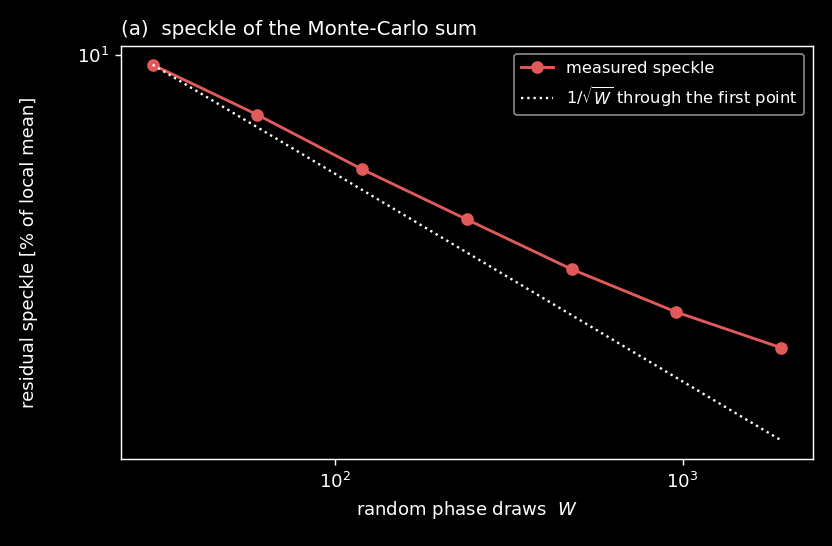
\includegraphics[width=0.5\textwidth]{mc.png}
\caption*{\textbf{Figure 1.} Residual speckle of the Monte-Carlo average against the
number of random phase draws, detector off, against a $1/\sqrt{W}$ reference.}
\end{figure}

\begin{figure}[t]
\centering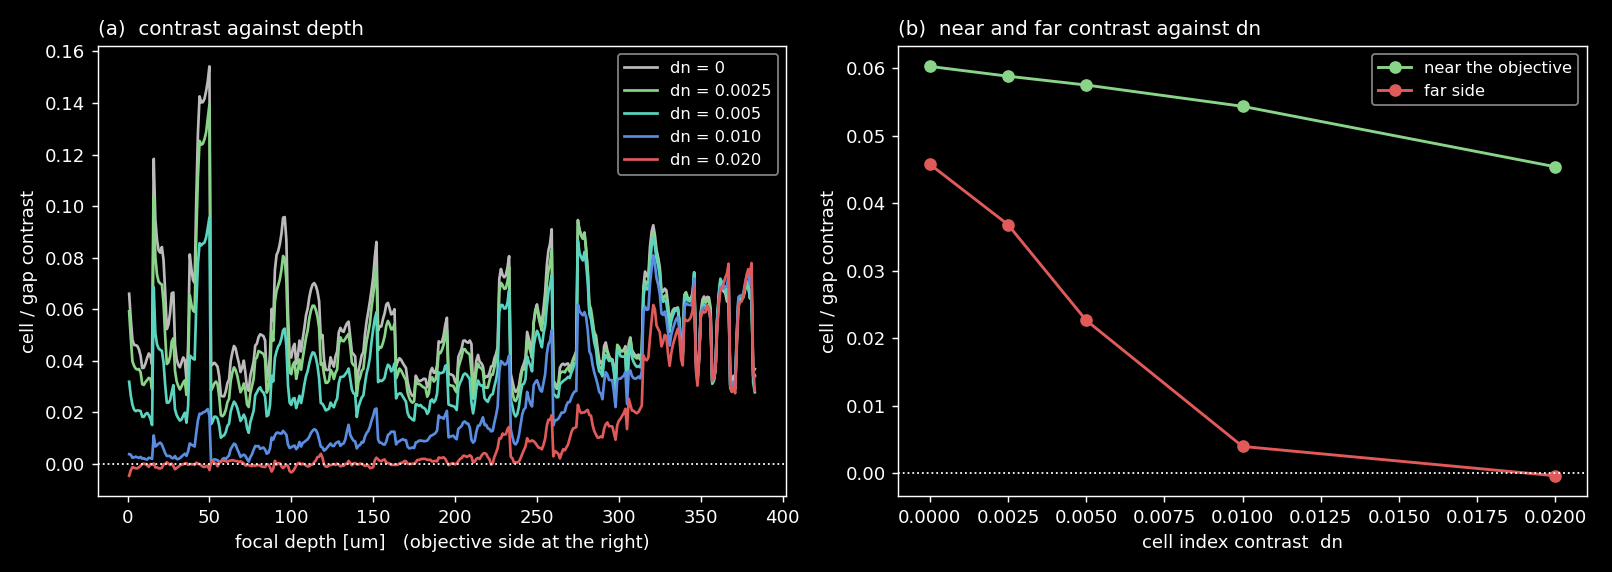
\includegraphics[width=\textwidth]{ri.png}
\caption*{\textbf{Figure 2.} Index sweep, 384\,\textmu m deep, no measurement noise.
(a) Cell/gap contrast against focal depth. (b) The same near the objective and on the
far side, against $dn$; the dotted line is zero contrast.}
\end{figure}

\begin{figure}[t]
\centering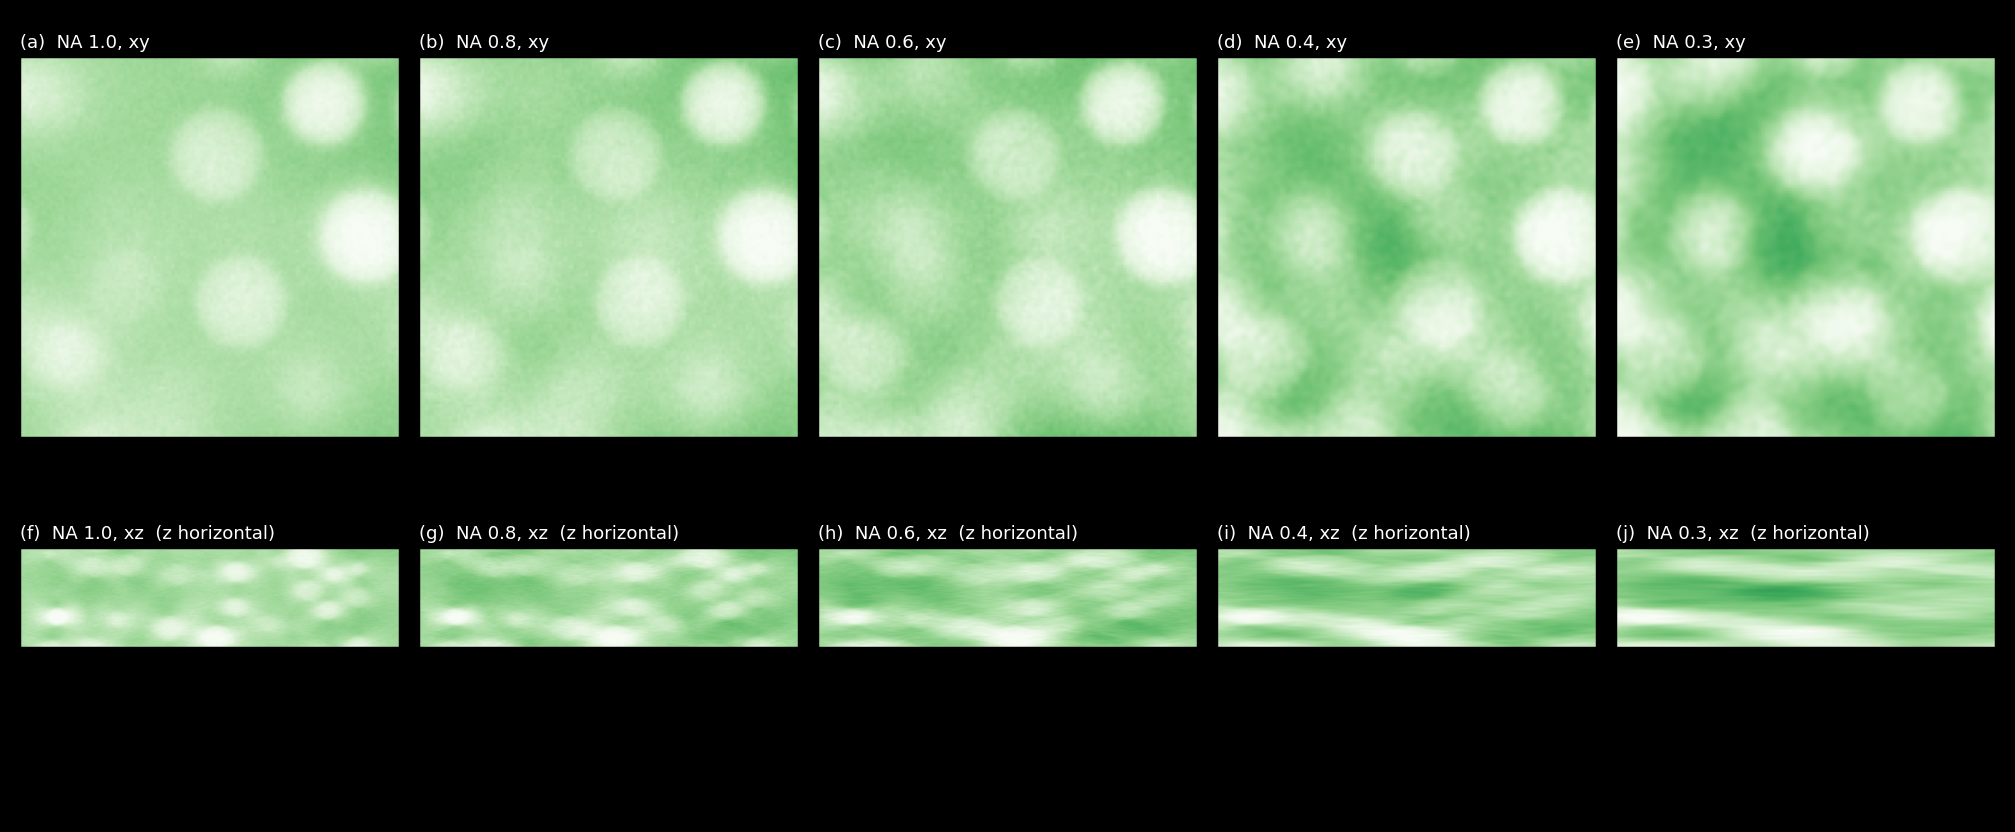
\includegraphics[width=\textwidth]{psf.png}
\caption*{\textbf{Figure 3.} NA sweep. Top row $xy$ sections, bottom row $xz$ sections
of the same volume, at the delivered voxel aspect. Lower NA leaves $xy$ nearly
unchanged and stretches $z$.}
\end{figure}

\begin{figure}[t]
\centering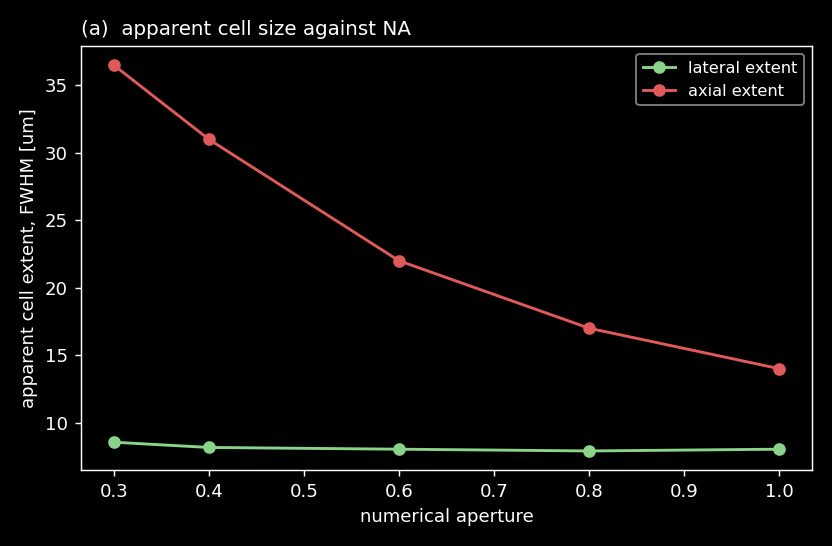
\includegraphics[width=0.5\textwidth]{psf_extent.png}
\caption*{\textbf{Figure 4.} Apparent cell extent, measured at half maximum through
each cell's own centre, against NA.}
\end{figure}

\end{document}
